\section{Utilisation type}
Dans cette partie sera évoqué un exemple d'utilisation type du programme.
Les actions de l'utilisateur serons décrites, et les processus techniques (en italique) que l'action engendre également. 

Notez que cette utilisation type se base sur des fonctionnalités de priorité 3 et 4.
Il est donc probable que l'application ne permette finalement pas toutes ces fonctionnalités. 

\subsection{Récupération des ISBN}

À la première utilisation du programme, l'adresse email à utiliser pour la synchronisation est demandée à l'utilisateur.
\emph{Au lancement du programme, celui - ci vérifiera l'existence d'un fichier de configuration contenant les caractéristiques de connexion à la boite email.
	Si ce fichier n'existe pas, il sera directement proposé au client de renseigner ces informations.}

L'utilisateur pourra aussi choisir d'utiliser l'adresse email liée au compte Android par défaut.
Ensuite, c'est une fenêtre à deux boutons qui se présente à l'utilisateur. 
Sur le premier est indiqué « Scanner un seul ouvrage », sur le second, « Scanner un lot d'ouvrages ». 
Si l'utilisateur se tourne vers la seconde option, 
un message apparait, demandant de viser le code barre du livre avec la caméra de l'appareil.
Il faut appuyer sur « ok », puis, l'appareil photo s'allume. 
\emph{C'est en fait à ce moment que Royal fait appel à la librairie ZXing afin de récupérer le code barre du livre, et d'en déduire l'ISBN.} 
L'utilisateur prend donc en photo le code barre du livre.
Un message s'affiche à présent à l'écran, avec marqué dessus « Vérification du livre » avec une barre de progression en dessous.
\emph{Le programme tente en fait d'interroger Google Book pour voir si des informations sur l'ouvrage sont disponible.}

Une fois la barre remplie, une autre phrase s'affiche : « Ouvrage identifié : < Nom de l'ouvrage> » la remplacera.
Ensuite un autre apparait demandant si c'est la fin du lot, ou si, au contraire, d'autres livres restent à scanner. 
\emph{Les ISBN, avec le nom de la bd sont écrits les un à la suite de l'autre dans un fichier.} 

L'utilisateur opte pour le second cas, afin d'enregistrer mes trois autres bd dans le logiciel. 
Malheureusement, arrivé au dernier, le portable lui indique que l'ouvrage est introuvable et lui demande donc de rentrer à la main le titre du livre. 
\emph{Le nom du livre est contenu dans le client Androïd, en plus du numéro d'ISBN pour que, une fois sur le client lourd,
	l'utilisateur sache encore de quel livre il s'agit sans pour autant avoir besoin de comparer l'ISBN.}

Une fois toutes les bd de scannés, l'utilisateur choisi de terminer l'enregistrement. 
\emph{À ce moment là, la date du scann est ajoutée au début du fichier contenant les ISBN.}

Peu de temps après, un nouveau message apparait : « Un e-mail de synchronisation a bien été envoyé sur votre boite mail, veuillez effectuer un import depuis votre ordinateur ».
\emph{Le fichier précédemment créé avec la date du scann, le numéro d'ISBN et le titre du livre est envoyé par e-mail à l'adresse définie pour l'exportation. 
	Le titre du mail correspond à une chaine identifiable par le client lourd : \textbf{Royal\_}
}

\subsection{Utilisation de l'application sur ordinateur}
Au premier démarrage du client PC, l'utilisateur se retrouve de nouveau face à une fenêtre me demandant de choisir quelle adresse e-mail il allait utiliser pour la synchronisation avec le « client Androïd ». 
C'est la même adresse que toute à l'heure qui doit être renseignée ici.
\emph{À l'exécution du programme, le fichier de sauvegarde de configuration \textbf{resources/royal.properties} est lu. 
	Si les champs \textbf{email\_address}, \textbf{email\_port} et \textbf{email\_protocol} sont vides, 
	on propose à l'utilisateur de renseigner ces informations, soit de façon manuelle, 
	soit en choisissant simplement la configuration de base liée au compte Androïd du téléphone (l'adresse GMail de l'utilisateur, donc).
}

Ensuite nous arrivons sur la page centrale du programme.
Celle - ci ressemble à une liste sur la quelle tous livres de l'utilisateur sont répertoriés.
Elle est vide pour le moment, et les boutons de gestion sont bien visible sur la partie haute de la fenêtre. 
On y retrouve un bouton pour ajouter un ouvrage, pour en supprimer un, pour l'édition, et enfin pour l'importation. 

\begin{figure}
\begin{center}
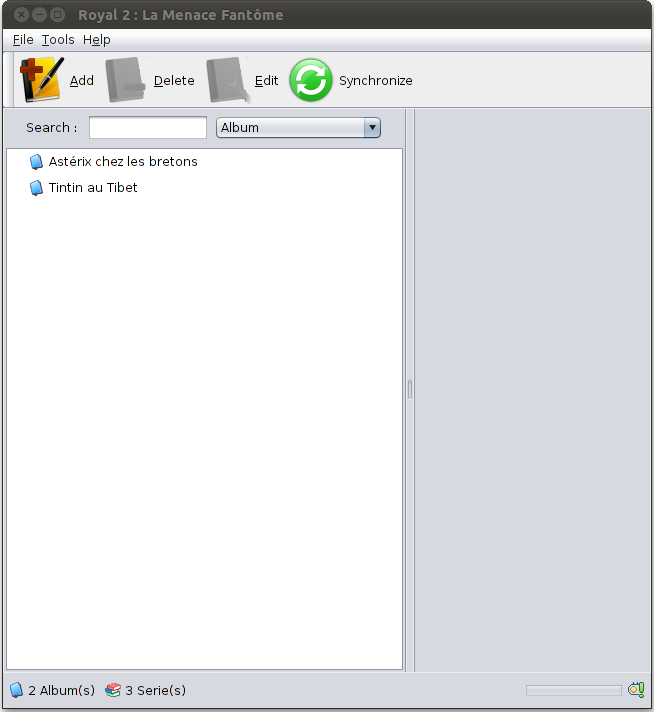
\includegraphics[height=10cm]{../img/principaleModifiee.png}
\end{center}
\caption{Page principale de l'application}
\end{figure}

Après un clique sur le bouton d'importation, 
une autre fenêtre apparait, indiquant d'attendre pendant l'opération. 
On peut voir en dessous une barre de progression, qui se remplie, au fur est à mesure de l'avancée des étapes : 
« Connexion au serveur mail », puis « Identification mail », après « Recherche des fichiers », et enfin « Téléchargement des ISBN ».
\emph{L'application va en effet se connecter sur la boite email de l'utilisateur et faire une recherche sur le sujet des messages contenus dans la boite de réception.
	Si un sujet est exactement composé de l'appellation « \textbf{Royal\_} », alors le contenu du message est téléchargé, et la recherche se termine.
	Il est à noter que chaque importation n'importera qu'un mail à la fois. 
	Le contenu du mail est ensuite traité : dans un premier temps la date de scann du lieux est conservé, puis chaque couple d'information (ISBN \slash{} Titre) pour chaque livre. 
}

Après ce temps d'attente, la fenêtre disparait, et une nouvelle affiche le récapitulatif des livres importés.
Le numéro ISBN est marqué dans une colonne, à côté, est écris « Téléchargement des informations », au fur est à mesure que le temps passe, les informations s'affichent pour chaque livre, sauf celui pour le quel un message d'erreur a été émis lors de la prise de photo de l'ISBN. 
L'utilisateur pourra toujours rentrer lui même les informations dans les champs laissés vide par défaut. 
\emph{C'est à ce moment que la recherche des informations sur les livres seront effectuées. 
	L'affichage sera évolutif, et l'API Google Dock sera interrogée pour chaque livre séparément. 
	Un message d'attente, ou de recherche en cours sera écrit pour les livres en attente de traitement. 
	Ceux dont une réponse de l'API sera déjà arrivé possèderons des champs éditables contenant par défaut les informations retournées, ou rien, si l'ISBN était introuvable. 
}

Une fois satisfait de la présentation de livre, il faut cliquer sur « Confirmer les informations des livres ». 
La prochaine fenêtre me demande si j'ai acheté ces ouvrages ou si je les ais empruntés dans une bibliothèque. 
On indiquera l'emprunt.

Le programme demandera ensuite dans quelle bibliothèque l'emprunt aura été effectué. 
Vu que l'installation est toute fraiche, aucune bibliothèque n'est existante pour le moment, la liste est vide.
Un bouton d'ajout sera à ce moment diponible. 
Un clique dessus produira l'ouverture d'une nouvelle fenêtre, demandant de renseigner le nom de la bibliothèque, son numéro de téléphone, la durée maximale de l'emprunt, et ses horaires d'ouverture. 
\emph{Les bibliothèques sont présentes dans une table à part de la base de données.
	À ce niveau, nous pouvons choisir de référer le lot à une bibliothèque déjà existante, ou à en créer une nouvelle
	(dans ce cas, une entrée sera évidemment créer dans la table des bibliothèques). 
	Notons que la notion de lot est quelque chose d'abstrait, d'un point de vue technique, aucune relation n'existe entre les livres.
	Il ne s'agit uniquement que d'un procédé évitant à l'utilisateur de renter des informations redondante pour chacun des livres.
	Ainsi, un identifiant vers la bibliothèque, et la date d'emprunt est conservé pour chaque livre.
}

De retour à la page principale de Royal, la liste des ouvrages que j'ai importé est à présent marquée dans la liste. 
Nous pouvons lire à droite quelques informations sur l'ouvrage sélectionné, dont la date de retour et la bibliothèque concernée. 

\begin{figure}[h]
\begin{center}
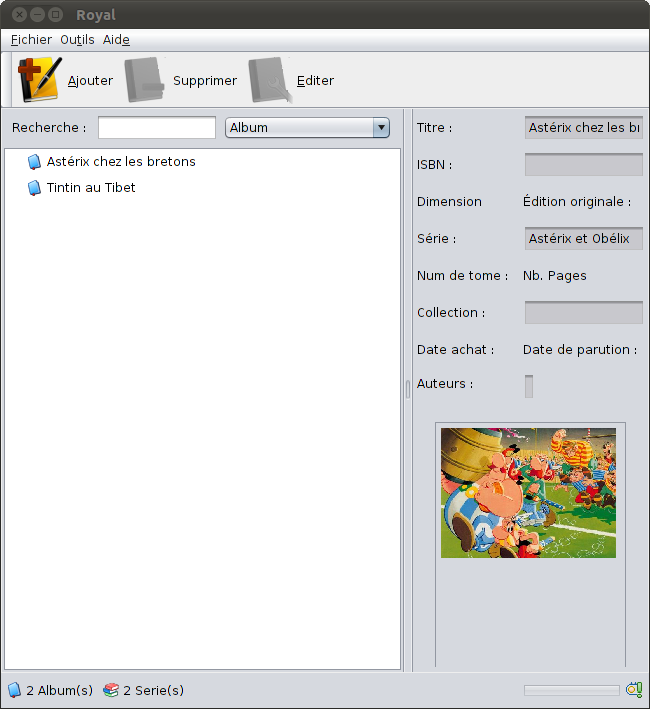
\includegraphics[height=10cm]{../img/principale.png}
\end{center}
\caption{Page principale du programme non vide}
\end{figure}

\subsection {Autres fonctionnalités}

\subsubsection {Scann d'un livre unique}
Nous choisirons cette fois le mode de scann simple, adapté pour un seul livre. 
L'appareil photo se rallume, on prend la photo du code barre, puis le nom de l'ouvrage réapparait sur l'écran.
On confirme, et l'exportation s'effectue apparemment avec succès. 
\emph{D'un point de vue interne au programme, le comportement est similaire entre le mode de scann par lot et celui par unité, la récursivité en moins.}

De retour devant l'ordinateur, nous ré effectuons une importation. 
Encore une fois, une fenêtre s'ouvre, avec les informations auto - complétées de l'ouvrage, il ne reste plus qu'à choisir la bibliothèque dans la quelle c'est effectué l'emprunt, à confirmer, et le livre s'ajoute dans la liste principale !

\subsubsection {Gestion des dates de retour}
Les dates de retour des ouvrages sont visibles dans les caractéristiques des livres. 
Un compte à rebours des jours restant avant la date critique sera aussi disponible dans la liste des livres.
Une alerte sera paramétrable dans les options permettant de rappeler à l'utilisateur les livres dont la date critique est proche, au démarrage de l'application.
Dans les informations sur l'œuvre, le client pourra, évidemment indiquer avoir rendu le livre.
Dans ce cas, plus aucune alerte ne sera émis sur le livre, ni d'affichage des jours restant.

\subsubsection {Modification des informations d'un livre}
Il suffira de cliquer sur le nom du livre qu'on comptera modifier pour voir un aperçu des informations contenues à son égard.
À ce moment, un bouton « Modifier » apparait en haut de la fenêtre.
Un clique sur celui - ci produira l'ouverture d'une nouvelle fenêtre donnant à l'utilisateur la possibilité de modifier toutes les informations.

\begin{figure}[h]
\begin{center}
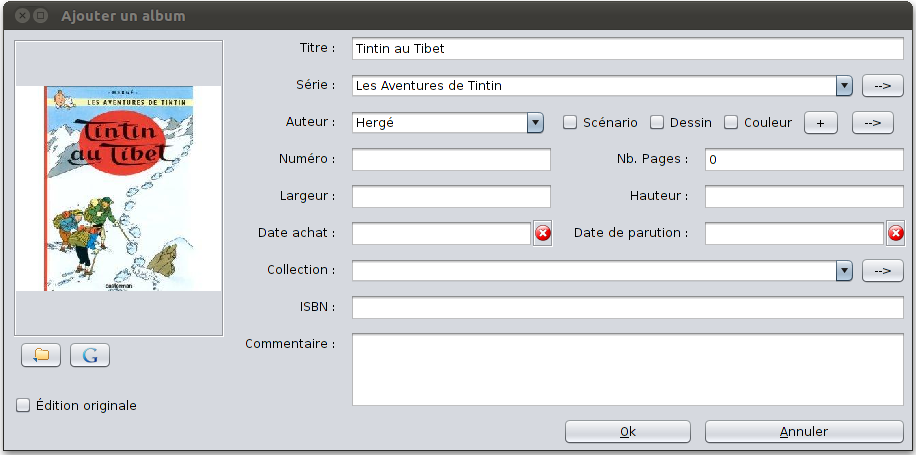
\includegraphics[height=5cm]{../img/editionAlbum.png}
\end{center}
\caption{Fenêtre d'édition des informations d'un livre}
\end{figure}
